\documentclass[english,11pt,a4paper]{article}

\newcommand\inner[2]{\langle #1, #2 \rangle} 

\newcommand{\R}{\mathbb{R}}

% ==============================================================================

%\usepackage{parskip}

\usepackage{a4wide}
\usepackage{tikz}
\usepackage{amsmath,epsfig,amssymb,amsbsy}
\usepackage{graphicx}
\usepackage{algorithm}
\usepackage{algpseudocode}

\usepackage[
	backend=biber,
	style=numeric,
	natbib=true,
	url=false, 
	doi=true,
	eprint=false
]{biblatex}

\addbibresource{references.bib}

\usepackage[
	a4paper, top=2.5cm, left=2cm, right=2.5cm
]{geometry}

\usepackage{enumitem}
\setlist[itemize]{noitemsep}

\usepackage[]{todonotes}

% ==============================================================================

\let\endtitlepage\relax
\endlinechar=-1

% ==============================================================================

\begin{document}

\begin{titlepage}
	\centering
	
	\includegraphics[width=0.25\textwidth]{images/Universitaet_Logo_RGB}\par
	\vspace{0.5cm}
	
	{\scshape \large Technical University of Munich \par}
	\vspace{0.5cm}
	
	{\bfseries \Large Optimization Algorithms for Deep Learning \par}
	{Interdisciplinary Project \par}
	\vspace{0.5cm}
	
	{Jens Gansloser \par}
	{Supervisor: Emanuel Laude \par}
	\vspace{0.5cm}
	
	{\today \par}
	\vspace{0.5cm}
\end{titlepage}

\section{Introduction}

Many complex tasks in engineering and science can be solved by learning a suitable model based on large training data sets with respect to some objective function. The state-of-the-art performing models often consist of deeply nested non-convex and non-smooth functions. With the increase in processing power it has recently become possible to train very deep models based on big datasets, often in a parallel manner. One example for these nested models are neural networks which are achieving high quality results in many application fields, often outperforming more classical methods. However, usually the training is done using stochastic gradient descent which is difficult to parallelize over layers and inhibits bad convergence properties. This work aims to compare different optimization algorithms to optimize deeply nested loss functions. As a baseline for comparing the algorithms we will use stochastic gradient descent. Important for comparisons are convergence properties and stability as well as the possibility to parallelize the algorithms.

\section{Objective Function}

In this work, the aim is to solve a supervised regression or classification problem involving a highly nested objective function. More specifically, a mapping $f(x)$ from the inputs $x$ to the corresponding outputs $y$ based on $N$ training samples $(x_n, y_n)$ should be learned. The problem can be written as

\begin{equation}
	\begin{aligned}
		& \underset{\{W_j\}}{\text{minimize}}
		& E(\{W_j\}) = \sum_{i=1}^{N} L(f(\{W_j\};x_i);y_i)
	\end{aligned}
	\label{eq:basis}
\end{equation}

with some suitable error measure $L(y_p;y)$ and model parametrization $\{W_j\}$. An example for an error measure is the squared l2-loss $L(y_p;y) = \frac{1}{2} \| y_p - y \|^2_2$ where $y_p$ is the model prediction and $y$ the ground truth data. The function $f(\{W_j\};x) = W_{K+1}h(W_Kh(\dots h(W_1x))$ is a nested K-layer mapping as it is usual in neural networks where $W_j$ are the weight matrices $W_1,\dots,W_{K+1}$ which do not need to have the same size. To keep the formulation clear, the biases are incorporated into the weight matrices. The nonlinear activation function $h(x)$ is applied element-wise and can also be non-differential. Examples are the sigmoid function $h(x) = 1/(1 + e^{-x})$ or the ReLU $h(x) = \mathrm{max}(0, x)$. Note that the sum over all samples can also be omitted by reformulating the involved functions to act on all training data simultaneously.

\section{Stochastic Gradient Descent}

The standard way of training neural networks is stochastic gradient descent. The gradient descent algorithm is used to find locally optimal parameters $\{W_j\}$. Here, in each step the gradient is calculated using the backpropagation algorithm and a fixed, randomly chosen number of samples from the training data. The network parameters are then updated using a fixed or diminishing stepsize. Note that in the case of stochastic gradient descent, using methods like Armijo linesearch does result in unstable behavior. While this method works often well in practice, it has only linear convergence and the tendency to get stuck at local minima (in comparison to more sophisticated majorization approaches for example). Additionally, finding a suitable step size often involves some heuristics and validation methods. It is well known that backpropagation leads to the vanishing gradient problem and therefore to small gradients which in turn requires the step size to be rather large, possibly leading to divergence of the algorithm.

\section{Solution Concept}

The problems of gradient descent are tackled by using splitting based optimization algorithms \cite{carreira2014distributed,taylor2016training} which show promising results with regard to stability and convergence rate. Thus it seems reasonable to analyze and compare different, more sophisticated optimization algorithms to solve deeply nested loss functions. In the following the used algorithms are explained. In this work we focus on the squared l2 loss. Therefore, additionally to the splitting algorithm we will compare a batched version of the Levenberg-Marquardt method. In the following, we stack all input samples into the matrix $x$ where each column is one sample point. Similarly, the target variables are stacked into the matrix $y$. The error function $L$ now operates on matrices. This formulation is equal to the formulation above, however, the layers now operate on all the data simultaneously as shown in equation~\ref{eq:basis_l2}.

\begin{equation}
	E(\{W_j\}) = L(f(\{W_j\};x);y) = \frac{1}{2} \| f(\{W_j\};x) - y \|^2
	\label{eq:basis_l2}
\end{equation}

For simplicity, in the following we only write $f(\{W_j\})$ and $L(f(\{W_j\}))$ omitting the inputs $x$ and targets $y$. 

\subsection{Last-layer Splitting}
\label{sec:last-layer_splitting}

By splitting the loss function at the network output and introducing constraints we can reformulate problem~\ref{eq:basis} as

\begin{equation}
	\begin{aligned}
		& \underset{\{W_j\},z}{\text{minimize}}
		&& L(z) \\
		& \text{subject to}
		&& z = f(\{W_j\}).
	\end{aligned}
	\label{eq:last-layer_splitting_problem}
\end{equation}

The augmented Lagrangian of this equality constrained problem is

\begin{equation}
	\begin{aligned}
		\mathcal{L}(\{W_j\}, z, \lambda)
		&= L(z) + \inner{\lambda}{f(\{W_j\})-z} + (\rho/2)\| f(\{W_j\})-z \|^2 \\
		&= L(z) + (\rho/2) \| f(\{W_j\}) - z + (1/\rho) \lambda \|^2 - (1/(2 \rho)) \| \lambda \|^2.
	\end{aligned}
\end{equation}

Note that by adding a regularizer $R(\{W_j\}) = (1/2) \sum_{j} \| W_j \|^2$ for the weights we get the standard ADMM formulation. Applying dual ascent to problem~\ref{eq:last-layer_splitting_problem} yields

\begin{equation}
	\begin{aligned}
		\{W_j\}^{k+1} &:= \underset{\{W_j\}}{\text{arg min }} \mathcal{L}(\{W_j\}, z^k, \lambda^k) \\
		&:= \underset{\{W_j\}}{\text{arg min }} (\rho/2) \| f(\{W_j\}) - z^k + (1/\rho) \lambda^k \|^2 \\
	
		z^{k+1} &:= \underset{z}{\text{arg min }} \mathcal{L}(\{W_j\}^{k+1}, z, \lambda^k) \\
		&:= \underset{z}{\text{arg min }} L(z) + (\rho/2) \| f(\{W_j\}^{k+1}) - z + (1/\rho) \lambda^k \|^2 \\
		
		\lambda^{k+1} &:= \lambda^k + \rho (f(\{W_j\}^{k+1})-z^{k+1}).
	\end{aligned}
\end{equation}

The gradients of the two primal problems can be written as

\begin{equation}
	\begin{aligned}
		\nabla_z \mathcal{L} &= \nabla L(z) - \lambda^k - \rho (f(\{W_j\}^k) - z) \\
		\nabla_{W_j} \mathcal{L} &= \rho J_f(\{W_j\})^T (f(\{W_j\}) - z^k + (1/\rho) \lambda^k).
	\end{aligned}
\end{equation}

We denote the $\{W_j\}$ problem as primal 1, the $z$ problem as primal 2 and the $\lambda$ problem as dual. Instead of first performing primal 2 as it is usual in the ADMM framework, we first perform primal 1\todo{Why does it work?}. Additionally, we only solve primal 1 inexactly, for example by only doing few gradient descent steps. \\ \\

Note that in the case of the squared l2 loss, for a choice of $\rho=1$ the algorithm is equal to gradient descent. Considering an iteration $k$, for $z^{k+1} = \text{arg min } \mathcal{L}(\{W_j\}^{k+1}, z, \lambda^k)$ being a stationary point, the necessary first order optimiality condition hast to hold. Setting the gradient to zero gives $z^{k+1} - \lambda^k - y = \rho(f(\{W_j\}^{k+1}) - z^{k+1})$. The dual can be written as $\lambda^{k+1} - \lambda^k = \rho(f(\{W_j\})^{k+1} - z^{k+1})$. Therefore it holds that $y = z^{k+1} - \lambda^{k+1}$. Considering the next iteration $k+1$, the primal update for the network weights results then by setting $\rho=1$ in 

\begin{equation}
	\{W_j\}^{k+1} = \underset{\{W_j\}}{\text{arg min }} \mathcal{L}(\{W_j\}, z^k, \lambda^k)
	= \frac{1}{2} \|f(\{W_j\}) - y\|^2 = L(f(\{W_j\})).
\end{equation}

This holds for all iterations except for $k=1$.

\subsubsection{Batched Primal Updates}

The primal update for the network weights can be minimized using various solvers for non-linear problems. However, in practice the training data is too large for a full batch approach. For example, using Levenberg-Marquardt would include solving a system of linear equations involving a coefficient matrix $\mathrm{J}_f^T \mathrm{J}_f$ of size $Nd \times Nd$ with $d$ being the input data dimension. Therefore, we use a batched approach where in each iteration $k$ the primal update for the network weights is done in a batched fashion. The $z$ and $\lambda$ updates are done full batch. In the case of the squared l2 loss both can be solved in closed form. The batched splitting algorithm is shown in algorithm~\ref{alg:sb}.

\begin{algorithm}
	\caption{Batched last-layer splitting}
	\label{alg:sb}
	\begin{algorithmic}[1]
		\State $x \gets$ Inputs
		\State $y \gets$ Targets
		\State Initialize $\{W_j\}^0, z^0, \lambda^0$
		\State Choose $\rho \in \R$
		\For{$k = 0,1,2,\dots$}
			\State $x_k, y_k \gets$ \Call{nextbatch}{$x, y, k$}
			\State $\{W_j\}^{k+1} \gets$ \Call{primal1}{$x_k,y_k$}
			\State $z^{k+1} \gets$ \Call{primal2}{$x,y$}
			\State $\lambda^{k+1} \gets \lambda^k + \rho (f(\{W_j\}^{k+1};x)-z^{k+1})$
		\EndFor
	\end{algorithmic}
\end{algorithm}

\subsection{Levenberg-Marquardt}

The Levenberg-Marquardt algorithm can be used to iteratively solve the non-linear least squares problem shown in \ref{eq:basis_l2}. Here, in each iteration $f$ is linearly approximated by $f(\{W_j\}+\delta;x) \approx f(\{W_j\};x) + \mathrm{J}\delta$ where $\mathrm{J}$ is the Jacobian at $\{W_j\}$. In each iteration the linearized problem shown in equation~\ref{eq:linearized_ls} is solved for $\delta$.

\begin{equation}
	E(\{W_j\}+\delta) \approx \frac{1}{2} \|f(\{W_j\};x) + \mathrm{J}\delta - y\|^2
	\label{eq:linearized_ls}
\end{equation}

The normal equations yield

\begin{equation}
	(\mathrm{J}^T \mathrm{J}) \delta = \mathrm{J}^T(y - f(\{W_j\};x)).
\end{equation}

By adding a damping term to the coefficient matrix on the left-hand side (which is equal to adding a regularizer term of the weights to the original problem) we get the Levenberg-Marquardt algorithm shown in equation~\ref{eq:levenberg-marquardt}.

\begin{equation}
	(\mathrm{J}^T \mathrm{J} + \lambda I) \delta = \mathrm{J}^T(y - f(\{W_j\};x)).
	\label{eq:levenberg-marquardt}
\end{equation}

The parameters are update in each step according to $\{W_j\}^{k+1} = \{W_j\}^k + \delta$. To find a suitable damping parameter $\lambda$ trust-region or line search methods can be used.

\subsubsection{Batched Levenberg-Marquardt}

Levenberg-Marquardt can only applied efficiently when the dimension of the mapping $f$ is relatively small. However, in our case we have large training data sets, which results in very large Jacobians. Similar to the splitting algorithm used, we use a batched variant of the Levenberg-Marquardt algorithm where only a randomly sampled subset of the training data is used to calculate the Jacobian\todo{Convergence proof?}.

\section{Experiments}

For the experiments the well known MNIST data set is used. It consist of. For efficient matrix calculus and utilization of GPUs the \textit{pytorch} library is used. In the experiments we compared. Good stepsize parameters are empirically determined.

% ==============================================================================

\newpage

\section{Appendix}

\subsection{Backpropagation}

For a matrix $X$, $X_{ij}$ selects the element in row $i$ and column $j$. If only one index is present, depending on the subscript a matrix row or column is select. In this case, $X_i$ is row $i$, $X_j$ is column $j$. \\ \\

As baseline we train the loss function using gradient descent. To calculate the gradients $\nabla_{W}E(W)$ of the loss function $E(W)$ backpropagation is used. Starting from the definition of the loss function in equation~\ref{eq:basis} we can calculate the gradient for each sample separately by computing $\nabla_{W}L(f(W;x_i);y_i)$ and summing over all samples. In the following we consider $W_{jk}^l$ as the weight connecting neuron $k$ to neuron $j$ of layer $l$. The linearities in layer $l$ are written as $z^l = W^la^{l-1} + b^l$ operating on the activations $a^{l-1}$. The activations of layer $l$ are computed as $a^l = h(W^l a^{l-1} + b^l) = h(z^l)$ with activation function $h$. Additionally, we have used the explicit formulation with the bias being a separate variable. This could also be included in the weight matrix by augmenting the activation vector with one and augmenting the weight matrix with the bias vector as last column. Figure \ref{fig:backprop} shows the neural network model at a layer $l$. We introduce the convention of $E^l_a$ being the error function of layer $l$ given the activations and $E^l_z$ being the error function of layer $l$ given the linearities. This allows us to split the error function and use the chain rule for computing the derivatives. Using this formulation, the goal is to calculate $\nabla_{W}E(W,b)$ and $\nabla_{b}E(W,b)$. By fixing all remaining weights and biases and applying the chain rule we get

\begin{equation}
	\begin{aligned}
		\frac{\partial E(W_{jk}^l)}{\partial W_{jk}^l} &= 
		\frac{\partial E^l_a(a^l(z^l(W_{jk}^l)))}{\partial W_{jk}^l} =
		\frac{\partial E^l_a}{\partial a^l} \frac{\partial a^l}{\partial z^l} \frac{\partial z^l}{\partial W^l_{jk}} =
		\frac{\partial E^l_a}{\partial a^l_j} \frac{\partial a^l_j}{\partial z^l_j} \frac{\partial z^l_j}{\partial W^l_{jk}}, \\
		\frac{\partial E(b_j^l)}{\partial b_j^l} &=
		\frac{\partial E^l_a(a^l(z^l(b_j^l)))}{\partial b_j^l} =
		\frac{\partial E^l_a}{\partial a^l} \frac{\partial a^l}{\partial z^l} \frac{\partial z^l}{\partial b_j^l} =
		\frac{\partial E^l_a}{\partial a^l_j} \frac{\partial a^l_j}{\partial z^l_j} \frac{\partial z^l_j}{\partial b_j^l}.
	\end{aligned}
	\label{eq:backprop_chainrule}
\end{equation}

Note that $\frac{\partial z^l_i}{\partial W^l_{jk}} = 0$ and $\frac{\partial z^l_i}{\partial b_j^l} = 0$ for all $i \neq j$ and $\frac{\partial a^l}{\partial z^l}$ is a diagonal matrix. We now introduce for each layer the error variable (row vector)

\begin{equation}
	\begin{aligned}
		\delta^l_j &= \frac{\partial E^l_a}{\partial a^l_j} \frac{\partial a^l_j}{\partial z^l_j} =
		\frac{\partial E^l_a}{\partial a^l_j} h'(z^l_j), \\
		\delta^l &= \frac{\partial E^l_a}{\partial a^l} \frac{\partial a^l}{\partial z^l} =
		\frac{\partial E^l_a}{\partial a^l} h'(z^l) = \frac{\partial E^l_a}{\partial a^l} \odot H'(z^l)^T
	\end{aligned}
\end{equation}

with $h'(z^l)$ being the Jacobian, $H'(z^l)$ the element-wise applied derivative of the activation function and $\odot$ the element-wise product. Note that the Jacobian is a diagonal matrix and we therefore can rewrite the equation using the Hadamard product. By expanding the first term we see that

\begin{equation}
	\begin{aligned}
		\frac{\partial E^l_a(a^l_j)}{\partial a^l_j} &= 
		\frac{\partial E^{l+1}_z(z^{l+1}(a^l_j))}{\partial a^l_j} = 
		\frac{\partial E^{l+1}_z}{\partial z^{l+1}} \frac{\partial z^{l+1}}{\partial a^l_j} = 
		\delta^{l+1}W^{l+1}_{:,j}, \\
		\frac{\partial E^l_a(a^l)}{\partial a^l} &= \delta^{l+1}W^{l+1}.
	\end{aligned}
\end{equation}

This shows that we can recursively compute the error variable $\delta^l$ starting from the last layer $L$ by

\begin{equation}
	\begin{aligned}
		\delta^l = \delta^{l+1}W^{l+1} h'(z^l) = \delta^{l+1}W^{l+1} \odot H'(z^l)^T.
	\end{aligned}
\end{equation}

\begin{figure}[t]
	\centering
	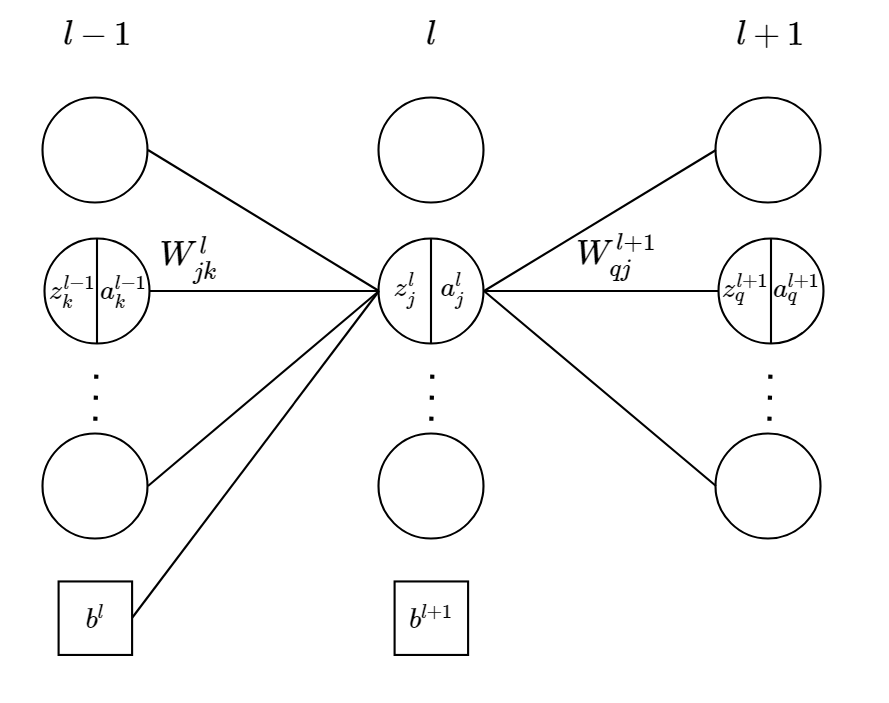
\includegraphics[width=0.6\textwidth]{images/backprop}
	\caption{Model of the neural network loss function with weights $W$, biases $b$, linearities $z$ and activations $a$ displayed at some layer $l$.}
	\label{fig:backprop}
\end{figure}

What remains is to compute the last terms of the equations \ref{eq:backprop_chainrule}. Since $\frac{\partial z^l_j}{\partial W^l_{jk}} = a^{l-1}_k$ and $\frac{\partial z^l_j}{\partial b_j^l} = 1$ we get

\begin{equation}
	\begin{aligned}
		\frac{\partial E(W_{jk}^l)}{\partial W_{jk}^l} &= \delta^l_j a^{l-1}_k, \\
		\frac{\partial E(b_j^l)}{\partial b_j^l} &= \delta^l_j.
	\end{aligned}
\end{equation}

Special care needs to be taken at the last layer of the network. Since it is usual to have only a linear layer at the end of a network without activation function the error variable (omitting the constants in the loss function) becomes 

\begin{equation}
	\begin{aligned}
		\delta^L = \frac{\partial L(z^L)}{\partial z^L} = \nabla L^T.
	\end{aligned}
\end{equation}

To efficiently implement backpropagation we can directly derive a matrix formulation so the iteration over all sample points is not required. By reformulating the loss function as $L(f(W;X);Y)$ with $X \in \R^{d \times N}, Y \in \R^{c \times N}, L: (\R^{c \times N},\R^{c \times N}) \to \R$, sample dimension $d$ and output dimension $c$ the activations and linearities are now matrices. To calculate the derivatives the involved matrices are vectorized in column-major order. Working through the stated derivation again but with the vectorized matrices we can rewrite the expressions in matrix form as

\begin{equation}
	\begin{aligned}
		\delta^l_m &= \delta^{l+1}_m W^{l+1} h'(z^l) = \delta^{l+1}_m W^{l+1} \odot H'(z^l)^T, \\
		\delta^L_m &= \text{reshape}(\frac{\partial L(z^L)}{\partial z^L}) = L_m, \\
		D_W^l &= \text{reshape}(\delta^l \mathrm{J}^l), \\
		D_b^l &= \sum_{i=1}^{N} (\delta^l_m)_{i}^T.
	\end{aligned}
\end{equation}

The gradients are represented by $\nabla_{W^l}E = D^l_W$ and $\nabla_{b^l}E = D^l_b$. Each row in the matrix $L_m$ is the transpose gradient w.r.t. each sample point $\nabla L(z^L_i)$. Each row of the matrix $H'$ is the derivative of the activation function applied element wise to the each sample point. For $D^l_b$ the summation is over the rows $i$ of the matrix $\delta^l_m$. Note that $D^l_W$ can be implemented faster using per element multiplication but is written in full matrix form for easier reading. The matrix $\mathrm{J}^l$ is the Jacobian $\frac{\partial z^l}{\partial W^l}$ with $W^l$ in row-major or column-major vectorization. In this formulation the vector version of the error variable $\delta^l$ is used. The reshape function extracts the rows and columns accordingly to get the matrix form.

\subsection{Softmax}

The softmax function is often used as last layer in classification tasks. It enables to interpret the neural network outputs as probabilities. The softmax function $\phi: \R^d \to [0,1]^d$ and its Jacobian are defined as

\begin{equation}
	\begin{aligned}
		\phi(x)_i &= \frac{e^{x_i}}{\sum_{j=1}^{d} e^{x_j}} \\
		\phi'(x) &= \text{diag}(\phi(x)) - \phi(x) \phi(x)^T
	\end{aligned}
\end{equation}

where $\sum_{i=1}^{d}\phi(x)_i = 1$. We also can write the softmax function in matrix form where $\phi$ is applied to each column of $x \in \R^{d \times N}$. The resulting Jacobian is then a block-diagonal matrix.

\subsection{Per-layer Splitting}

In comparison to the last-layer splitting explained in section~\ref{sec:last-layer_splitting} it is also possible to split the loss function at each layer. This section describes this approach. In the following, without loss of generality we consider a 2-layer neural network mapping $f(\{W_j\};x) = W_3h(W_2h(W_1x))$ with a linear mapping to the output variables. The unconstrained optimization problem can then be written as

\begin{equation}
	\begin{aligned}
		& \underset{\{W_j\}}{\text{minimize}}
		& & L(W_3h(W_2h(W_1x);y).
	\end{aligned}
	\label{eq:loss_function}
\end{equation}

To split the nested objective function we decouple the weights and activation functions by introducing additional variables and adding the appropriate constraints. Note that we omit the constant $y$ in the following equations for the sake of simplicity. By decoupling and introducing constraints we can reformulate problem \ref{eq:loss_function} as

\begin{equation}
	\begin{aligned}
		& \underset{\{W_j\},\{a_i\},z}{\text{minimize}} && L(z) \\
		& \text{subject to} & a_1 &= h(W_1x), \\
		&& a_2 &= h(W_2a_1), \\
		&& z &= W_3a_2
	\end{aligned}
\end{equation}

with the new variables $a_1, a_2, z$. The augmented Lagrangian of this equality constrained problem is

\begin{equation}
	\begin{aligned}
		\mathcal{L}(\{W_j\}, \{a_i\}, z, \{\lambda_j\}) = L(z) + 
		& \inner{\lambda_1}{h(W_1x)-a_1} + (\rho/2) \| h(W_1x)-a_1 \|^2 + \\
		& \inner{\lambda_2}{h(W_2a_1)-a_2} + (\rho/2) \| h(W_2a_1)-a_2 \|^2 + \\
		& \inner{\lambda_3}{W_3a_2-z} + (\rho/2) \| W_3a_2-z \|^2.
	\end{aligned}
\end{equation}

For minimizing the objective we update the weights and constraint variables of subproblems in an alternating fashion using gradient descent. In each update step we only consider the variables of one constraint and fix all other terms of the augmented Lagrangian. This results in one subproblem $\mathcal{H}_i$ for each constraint.

\begin{equation}
	\begin{aligned}
		\mathcal{H}_1(W_1,a_1,\lambda_1) &= && \inner{\lambda_1}{h(W_1x)-a_1} + (\rho/2) \| h(W_1x)-a_1 \|^2 + \\
		& && \inner{\lambda_2}{h(W_2a_1)-a_2} + (\rho/2) \| h(W_2a_1)-a_2 \|^2 \\
		\mathcal{H}_2(W_2,a_1,a_2,\lambda_2) &= && \inner{\lambda_2}{h(W_2a_1)-a_2} + (\rho/2) \| h(W_2a_1)-a_2 \|^2 + \\
		& && \inner{\lambda_1}{h(W_1x)-a_1} + (\rho/2) \| h(W_1x)-a_1 \|^2 + \\
		& && \inner{\lambda_3}{W_3a_2-z} + (\rho/2) \| W_3a_2-z \|^2 \\
		\mathcal{H}_3(W_3,a_2,z,\lambda_3) &= && \inner{\lambda_3}{W_3a_2-z} + (\rho/2) \| W_3a_2-z \|^2 + L(y,z) \\
		& && \inner{\lambda_2}{h(W_2a_1)-a_2} + (\rho/2) \| h(W_2a_1)-a_2 \|^2
	\end{aligned}
\end{equation}

We need to take special care of the first subproblem (constraint for the first layer) involving the input $x$ and the last subproblem (constraint for the last linear layer) involving the predicted variable $z$. For all others we consider the update scheme (here for $\mathcal{H}_2$)

\begin{equation}
	\begin{aligned}
		W_2^{k+1} &= W_2^k - \rho_1 \nabla_{W_2}(\mathcal{H}_2(W_2^k,a_1^k,a_2^k,\lambda_2^k)) \\
		a_1^{k+1} &= a_1^k - \rho_2 \nabla_{a_1}(\mathcal{H}_2(W_2^k,a_1^k,a_2^k,\lambda_2^k)) \\
		a_2^{k+1} &= a_2^k - \rho_3 \nabla_{a_2}(\mathcal{H}_2(W_2^{k+1},a_1^{k+1},a_2^k,\lambda_2^k)) \\
		\lambda_2^{k+1} &= \lambda_2^{k} + \rho (h(W_2^{k+1}a_1^{k+1})-a_2^{k+1})
	\end{aligned}
\end{equation}

which are gradient descent steps for the primal variables and gradient ascent steps for the dual variable $\lambda$. For $\mathcal{H}_1$ only $W_1$, $a_2$ and $\lambda_1$ need to be updated since $x$ is a constant. For the last subproblem $\mathcal{H}_{K+1}$ we need to add $\nabla_zL(z)$ to the gradient with respect to $z$.

\pagebreak

\printbibliography

\end{document}

